\chapter{Introduction}

\begin{quotation}[Título]{Autor}
Texto \\
Text
\end{quotation}

\noindent OLD:\{
\begin{enumerate}
  \item Reliability engineering
  \begin{enumerate}
    \item Describe safety (related to lives), reliability (related to cost).
  \end{enumerate}
  \item Fault tolerance
  \begin{enumerate}
    \item Definition
    \item Patterns
  \end{enumerate}
  \item Functions to describe component behaviour. Include time
  \item Make a ft-pattern replaceable by its function refinement.
\end{enumerate}
\}

%\usepackage{graphics} is needed for \includegraphics
\begin{figure}[htp]
\begin{center}
  % \begin{tikzpicture}[
% block/.style={ellipse, draw, fill=yellow!20, rounded corners=.8ex, inner sep=5pt},
% edgedesc/.style={rectangle, draw, fill=blue!10, rounded corners=.8ex, inner sep=5 pt},
% every label/.style={gray, font=\scriptsize}
% ]
% \node (system) [block] {System};
% \node (faultmodel) [block, below left=2cm and 3cm of system, label={below right: fault modelling}] {System Fault Model};
% \node (structurefSFM) [block, below=3cm of faultmodel] {Structure function};
% \node (faulttree) [block, below right=2cm and 3cm of system] {Fault Tree};
% \node (structurefFT) [block, below=3cm of faulttree] {Structure function};
% 
% 
% \draw [->] (system) -| node[edgedesc] {%
% \begin{minipage}{0.3\textwidth}
% Abstracts nominal values to ``Nominal'', faults are in library components, and the library is extensible.
% \end{minipage}
% } (faultmodel);
% \draw [->] (system) -| node[edgedesc, fill=red!20] {Conforms to} (faulttree);
% \draw [->] (faultmodel) -- node[edgedesc] {%
% \begin{minipage}{0.3\textwidth}
% By composition of library components and simplification.
% \end{minipage}
% } (structurefSFM);
% \draw [->] (faulttree) -- (structurefFT);
% \draw [<->] (structurefSFM) -- node [edgedesc, fill=green!20] {Adherence} (structurefFT);
% \end{tikzpicture}
%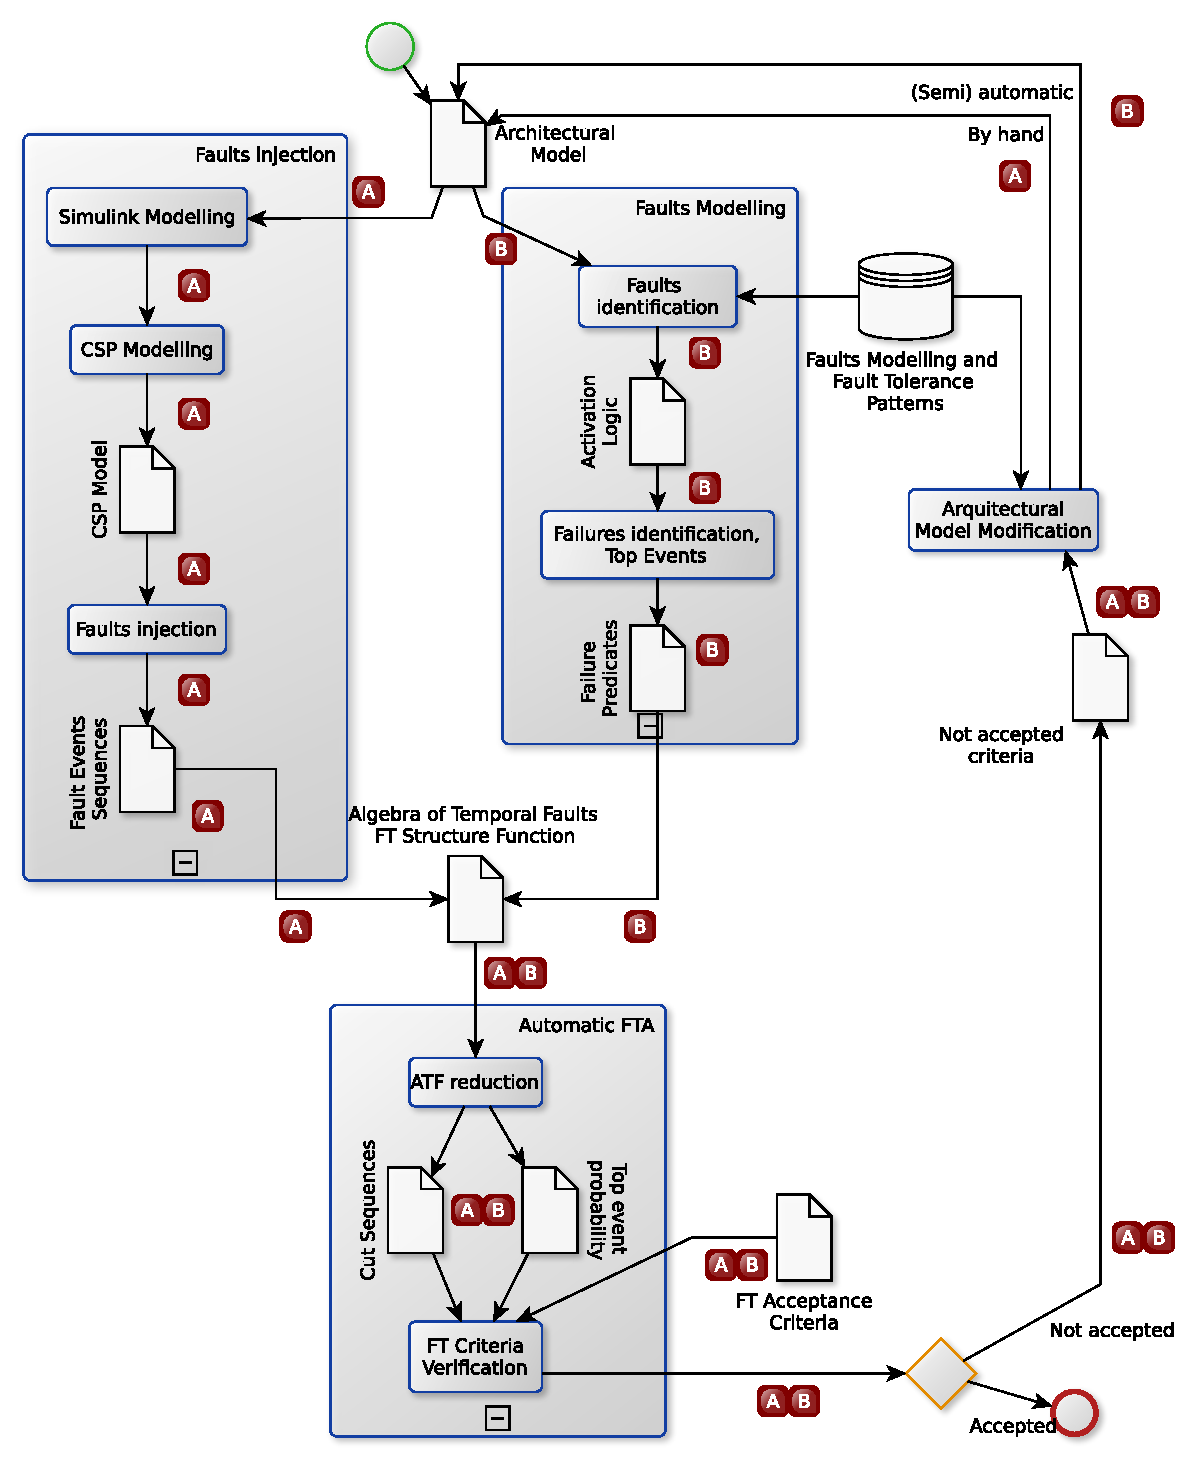
\includegraphics[width=0.5\textwidth]{StrategyOverview.eps}
%\includegraphics[width=0.5\textwidth]{temp.png}
  \caption{Overview}
  \label{fig:overview}
\end{center}
\end{figure}